
\documentclass[journal]{IEEEtran}

\IEEEoverridecommandlockouts                              % This command thanks command
%\overrideIEEEmargins
% See the \addtolength command later in the file to balance the column lengths
% on the last page of the document

%\def\baselinestretch{0.9999}

%\input{boldfacemath}

%\usepackage{exsheets}



% save and then undefine the offending command
% we need \makeatletter because \@undefined uses the special @ character.
\makeatletter
\let\IEEEproof\proof
\let\IEEEendproof\endproof
\let\proof\@undefined
\let\endproof\@undefined
\makeatother

% The following packages can be found on http:\\www.ctan.org
%\usepackage{graphics} % for pdf, bitmapped graphics files
%\usepackage{epsfig} % for xpostscript graphics files
%\usepackage{mathptmx} % assumes new font selection scheme installed
%\usepackage{times} % assumes new font selection scheme installed
\usepackage{amsmath} % assumes amsmath package installed
\usepackage{amssymb}  % assumes amsmath package installed
\usepackage{amsthm}
\usepackage{amsfonts}
\usepackage{mathtools}

% Text
\usepackage{comment}
\usepackage[normalem]{ulem}
%\usepackage[inline]{enumitem}
%let\labelindent\relax % Since the \labelindent command exists for legacy reasons in the IEEE template, you can simply "disable" it by adding the following before importing the enumitem package
%\usepackage{enumitem}
\usepackage{bm}
\providecommand{\bm}{\pmb}

%\usepackage{flushend}

\newtheorem{prop}{Proposition}
\newtheorem{cor}{Corollary}
\newtheorem{defin}{Definition}
\newtheorem{fact}{Fact}
\newtheorem{thm}{Theorem}[section]
\newtheorem{lem}[thm]{Lemma}
\newtheorem*{Zorn}{Zorn’s Lemma}
\theoremstyle{definition}
\newtheorem{dfn}{Definition}
\theoremstyle{remark}
\newtheorem*{rmk}{Remark}
\newtheorem{theorem}{Theorem}[section]
\newtheorem{remark}[theorem]{Remark}

\newtheorem{problem}{Problem}

\usepackage{verbatim}

\usepackage{color}
%\usepackage{subfig}
\usepackage{graphicx}
%\usepackage{caption}
\usepackage{esvect}



%\usepackage{mathptmx}
\usepackage{times}

%%%%%%%%%%%%%%%%%%%%%%%%%%%%%%%%%%%%%%%%%%%%%

\usepackage[ruled,vlined,linesnumbered]{algorithm2e}
%\usepackage[noend]{algorithmic}
\usepackage{algorithmicx}
\usepackage{algpseudocode}

%%%%%%%%%%%%%%%%%%%%%%%%%%%%%%%%%%%%%%%%%%%%%
\graphicspath{{images/}}

\usepackage[us]{datetime}
\usepackage{caption}
\captionsetup{font=small}


%\documentclass[a4, 10pt, conference]{ieeeconf}

 \usepackage[usenames,dvipsnames,table]{xcolor}

\usepackage{hyperref} %pdf with links and toc on the left
\hypersetup{
    colorlinks,
    citecolor=black,
    filecolor=black,
    linkcolor=black,
    urlcolor=black,
    pdfauthor={},
    pdfsubject={},
    pdftitle={}
}

\usepackage{todonotes}
%\usepackage{todonotes} lets you insert notes of stuff to do with the syntax \todo{Add details.}

\usepackage{graphicx}
% \usepackage{graphicx} manage external pictures

\usepackage{latexsym}
\usepackage{color}
% \usepackage{color} adds support for colored text

\usepackage{cite}

% \usepackage{cite} assists in citation management

\usepackage{caption}
%\usepackage{caption} allows customization of appearance and placement of captions for figures, tables, etc.
\usepackage{subcaption}
%\usepackage{subfigure}


\usepackage{tikz}
\usepackage{adjustbox}
\usetikzlibrary{shapes,arrows}

% ---------- added packages -----------------------------------
\usepackage{tabularx, booktabs}
\newcolumntype{Y}{>{\centering\arraybackslash}X}
\usepackage{multirow}
\usepackage{paralist}
\usepackage{booktabs}
%\usepackage[table,xcdraw]{xcolor}
% ---------- New Symbols and Commands -------------------------
\usepackage{accents}
% ---------- Standard Commands ------------------

\usepackage{color}
\newcommand\red[1]{{\textcolor{red}{#1}}}
\newcommand\blue[1]{{\textcolor{blue}{#1}}}

\newcommand{\DS}[1]{\red{DS: #1}}
\newcommand{\MANU}[1]{\blue{MANU: #1}}
% ---------- new variables ------------------
\newcommand{\Hinf}{$H_\infty$\xspace}
\newcommand{\photoa}{PH-A}
\newcommand{\photob}{PH-B}
\newcommand{\photodistance}{d}


% ---------- new commands ------------------
\newcommand{\vect}[1]{\bm{#1}}		% vectors
\newcommand{\matr}[1]{\bm{#1}}		% matrices
\newcommand{\nR}[1]{\mathbb{R}^{#1}}		% real number
\newcommand{\nT}[1]{\mathbb{T}^{#1}}		% real number
\newcommand{\define}{:=}			% define symbol
\newcommand{\modulus}[1]{\left| #1 \right|}	% abs
\newcommand{\matrice}[1]{\begin{bmatrix} #1 \end{bmatrix}}	% matrix
\newcommand{\smallmatrice}[1]{\left[\begin{smallmatrix} #1 \end{smallmatrix}\right]}	% matrix
\newcommand{\cosp}[1]{\cos \left( #1 \right)}	% cos with brace
\newcommand{\sinp}[1]{\sin \left( #1 \right)}	% sin with brace
\newcommand{\determinant}[1]{\text{det}\left(#1\right)} 	% determinant
\newcommand{\sgn}[1]{\text{sgn}\left( #1 \right)}			% signum
\newcommand{\atanTwo}[1]{{\rm atan2}\left( #1\right)}		% atan2
\newcommand{\acotTwo}[1]{{\rm acot2}\left( #1\right)}		% acot2
\newcommand{\upperRomannumeral}[1]{\uppercase\expandafter{\romannumeral#1}}	% roman numbers
\newcommand{\lowerromannumeral}[1]{\romannumeral#1\relax}
\newcommand{\vSpace}{\;\,}
\newcommand{\ubar}[1]{\underaccent{\bar}{#1}}

%-----------Functions------------------------
\newcommand{\minEig}[1]{\lambda_{\text{min}}[#1]}
\newcommand{\maxEig}[1]{\lambda_{\text{max}}[#1]}
\newcommand{\transp}{^\top}


% --------- References ----------------------
\newcommand{\fig}{Fig.~}	% figure ref
\newcommand{\eqn}{Eq.~}	% equation ref
\newcommand{\tab}{Tab.~}	% table ref
\newcommand{\cha}{Chap.~}	% chapter ref
\newcommand{\sect}{Sec.~}	% section ref
\newcommand{\alg}{Algorithm~}

% --------- Variables -----------------------

% General
\renewcommand{\frame}{\mathcal{F}}		% frame
\newcommand{\origin}{O}						% origin
\newcommand{\vX}{\vect{x}}					% x-axis
\newcommand{\vY}{\vect{y}}					% y-axis
\newcommand{\vZ}{\vect{z}}					% z-axis
\newcommand{\pos}{\vect{p}}				% position vector
\newcommand{\dpos}{\vect{v}}				% velocity vector
\newcommand{\rotMat}{\matr{R}}				% rotation matrix
\newcommand{\rotMatVectAngle}[2]{\rotMat_{#1}(#2)}	% rotation matrix representing the rotation about a vector of a certain angle
\newcommand{\vZero}{\vect{0}}				% vect/matr of zeros
\newcommand{\en}[1]{\vect{e}_{#1}}		% vect e_n
\newcommand{\eye}[1]{\matr{I}_{#1}}
\newcommand{\zeros}[1]{\matr{0}_{#1}}
\newcommand{\skewmatr}[1]{\big[{#1}\big]_\times}
\newcommand{\skewmatrS}[1]{\matr{S}({#1})}

% World frame
\newcommand{\frameW}{\frame_W}			% world frame
\newcommand{\originW}{\origin_W}		% origin world frame
\newcommand{\xW}{\vX_W}				% x-axis world frame
\newcommand{\yW}{\vY_W}				% y-axis world frame
\newcommand{\zW}{\vZ_W}				% z-axis world frame
\newcommand{\dxW}{\dot{\vX}_W}

% Background
\newcommand{\samplingPeriod}{T_s}
\newcommand{\samplingFrequency}{f_s}
\newcommand{\vwater}{\bar{v}_{water}}
\newcommand{\vhex}{\bar{v}_{hex}}
\newcommand{\vfluid}{\bar{v}_{fl}}
\newcommand{\samplesWater}{N_{water}}
\newcommand{\samplesHex}{N_{hex}}
\newcommand{\samplesfl}{N_{fl}}
\newcommand{\samplesflk}{N_{fl,k}}
\newcommand{\samples}{n}
\newcommand{\avgL}[1]{L_{#1}}
\newcommand{\vnominal}{v_{n}}
\newcommand{\channelArea}{A}
\newcommand{\slugvelocity}{v_{sl}}


% Modeling 2nd Order Systems
\newcommand{\settlingtime}{t_s}
\newcommand{\naturalfrequency}{w_n}
\newcommand{\damping}{\xi}
\newcommand{\bias}{b_{0}}

% Modeling
\newcommand{\eigenvalues}[1]{\lambda_{#1}}
\newcommand{\slugfrequencyerror}{e_{\slugfrequency}}

% Flow rates
\newcommand{\flowratecommand}{F^{\star}_{fl}}
\newcommand{\flowrate}{F}
\newcommand{\flowratewatercommand}{F^{\star}_{water}}
\newcommand{\flowratehexcommand}{F^{\star}_{hex}}
\newcommand{\urate}{u_{fl}}
\newcommand{\uratess}{\expectedflowrate}
\newcommand{\urateinit}{u_{fl_{0}}}

\newcommand{\uratecommand}{\urate^{\star}}
\newcommand{\uratecommandwater}{u^{\star}_{water}}
\newcommand{\uratecommandhex}{u^{\star}_{hex}}
\newcommand{\out}{y}


% Frequency
\newcommand{\slugfrequency}{f_{sl}}
\newcommand{\slugfrequencyinit}{f_{sl_{0}}}
\newcommand{\slugfrequencyss}{\tilde{f}_{sl}} %steady-state
\newcommand{\currentslugfrequency}{f_{sl}^c}
\newcommand{\desiredslugfrequency}{f_{sl}^d}
\newcommand{\slugfrequencyDes}{\desiredslugfrequency} %easy to use command wrt desiredsslugfrequency. This is the reason of the repetition.

% Control
\newcommand{\samplesk}{k}
\newcommand{\modelgain}{K_p}
\newcommand{\predictionHorizon}{N_p}
\newcommand{\controlHorizon}{N_c}
\newcommand{\controlVector}{\Delta \matr{U}}
\newcommand{\controlvector}[1]{\Delta \uratecommand({#1})}
\newcommand{\controlsample}{\uratecommand}
\newcommand{\referenceVector}{\matr{R}_{\slugfrequency}}
\newcommand{\outputVector}{\matr{Y}}
\newcommand{\outputvector}[1]{y_{fl}(#1)}
\newcommand{\costfunction}{\matr{J}}
\newcommand{\performanceMatrix}{\bar{\matr{R}}}
\newcommand{\slugfrequencymean}{\mu_{\slugfrequency}}
\newcommand{\slugfrequencystd}{\sigma_{\slugfrequency}}
\newcommand{\expectedflowrate}{\tilde{u}_{fl}}

\newcommand{\transitionMatrix}{\matr{F}}
\newcommand{\controlMatrix}{\matr{\Phi}}
\newcommand{\state}{x} 
\newcommand{\timeWindow}{t_w}


%My symbols
\newcommand{\abscissa}{x}
\newcommand{\ordinate}{y}
\newcommand{\mean}[1]{<V_{#1}(t)>}
\newcommand{\meann}{<V(t)>}
\newcommand{\spatialmean}[3]{V_{#1}({#2},{#3},t)}
\newcommand{\width}{W_{ROI}}
\newcommand{\height}{H_{ROI}}
\newcommand{\frequency}{f_i}
\newcommand{\amplitude}{A}
\newcommand{\range}{Range<V_x(t)>}
\newcommand{\peak}{AP}
\newcommand{\particles}{<N_p(t)>}

%Measurement units
\newcommand{\pixel}{pixels}
\newcommand{\apixel}{pixel}
\newcommand{\density}{Kg/m^3}
\newcommand{\hertz}{Hz}
\newcommand{\flow}{ml/min}
\newcommand{\seconds}{s}
\newcommand{\framerate}{FPS}
\DeclarePairedDelimiter{\norm}{\lVert}{\rVert} % norm

\captionsetup[subfigure]{labelformat=simple, labelsep=colon}
\makeatletter
\renewcommand*{\thesubfigure}{(\alph{subfigure})} 
\makeatother
%\makeatother
\pagestyle{headings}

%%%%%%%%%%%%%%%%%%%%%%%%%%%%%%%%%%%%%%%%%%%%%%%%%%%%%%%%%%%%%%%%%%%%%%%%%%%%%%%

\title{DPIV Analysis and Real Time Implementation}


\author{E. Cutuli${^{1}}$, G. Stella${^{1}}$, D. Sanalitro${^{1}}$, M. Bucolo${^{1}}$~\IEEEmembership{Senior Member,~IEEE}

\thanks{$^1$Department of Electrical Electronic and Computer Science Engineering, University of Catania, CT, Italy. {\tt \scriptsize\href{mailto:uni391076@studium.unict.it}{\mbox{uni391076@studium.unict.it}}
\scriptsize\href{mailto:emaunuela.cutuli@phd.unict.it}{\mbox{emanuela.cutuli@phd.unict.it}}
\scriptsize\href{mailto:giovanna.stella@phd.unict.it}{\mbox{giovanna.stella@phd.unict.it}}
\scriptsize\href{mailto:dario.sanalitro@unict.it}{\mbox{dario.sanalitro@unict.it}}}. 
\scriptsize\href{mailto:maide.bucolo@unict.it}{\mbox{maide.bucolo@unict.it}}}. 
}

%\thanks{Digital Object Idenitifier (DOI): see top of this page}




%%%%%%%%%%%%%%%%%%%%%%%%%%%%%%%%%%%%%%%%%%%%%%%%%%%%%%%%%%%%%%%%%%%%%%
\begin{document}
%%%%%%%%%%%%%%%%%%%%%%%%%%%%%%%%%%%%%%%%%%%%%%%%%%%%%%%%%%%%%%%%%%%%%%


\maketitle

%%%%%%%%%%%%%%%%%%%%%%%%%%%%%%%%%%%%%%%%%%%%%%%%%%%%%%%%%%%%%%%%%%%%%%
\begin{abstract}

\end{abstract}
%%%%%%%%%%%%%%%%%%%%%%%%%%%%%%%%%%%%%%%%%%%%%%%%%%%%%%%%%%%%%%%%%%%%%%

\begin{IEEEkeywords}
	Signal processing, Micro-optofluidic device, Data-driven Modelling
\end{IEEEkeywords}

\section{Introduction}

This paper ecc...

\subsection{Paper main contributions}


\section{Materials and Methods}
This chapter of the paper is organized as follow. \sect\ref{sec:design} provides a schematic description of the hardware platform realization, \sect\ref{sec:method} describes the applied methodology and in \sect\ref{sec:setup} the experimental setup and campaigns are presented.

\subsection{System Design and Hardware Platform Realization}\label{sec:design}

\begin{figure*}[t]
	\centering
	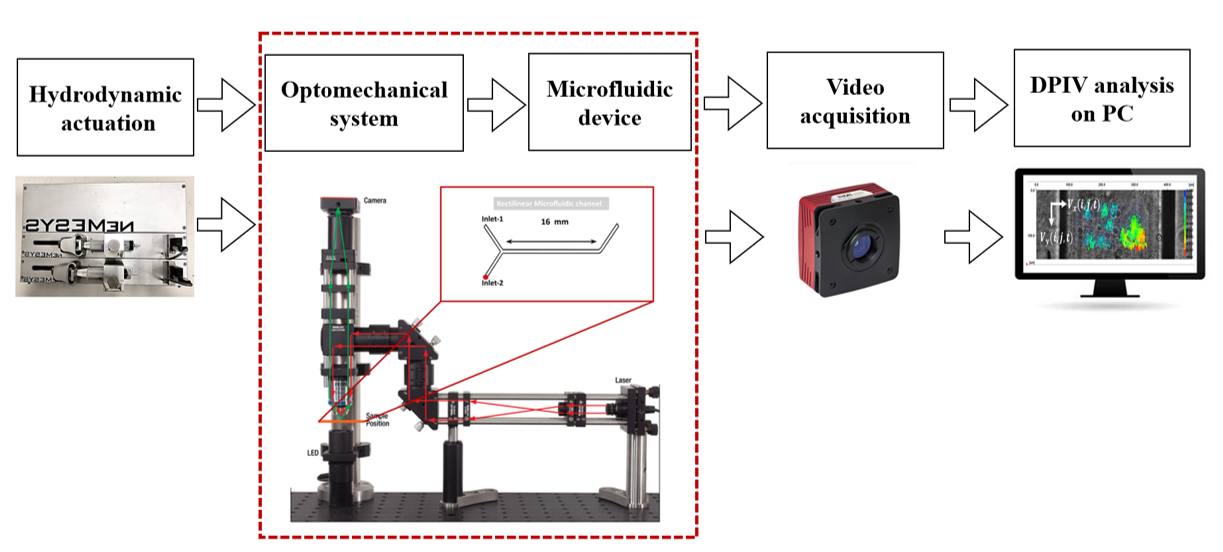
\includegraphics[width=2\columnwidth]{images/PlatformDesign}
	\centering{\caption{\label{Platform}System Design and Hardware Platform Realization block schemes.}}
\end{figure*}

From a methodological point of view, the experimental characterization of the process takes place through the acquisition of videos that allow studying different interaction mechanisms between particles/cells subjected to different external stresses.
The captured videos are then analyzed using Digital Particle Image Velocimetry (DPIV).
In order to study the different interaction mechanisms between particles in micro-channels subject to external hydrodynamic actuation, the system is composed of i) the hydrodynamic actuation system, ii) the optomechanical system, iii) the microfluidic device,, iv) a video-acquisition system, v)  a PC where the algorithm runs, as shown in \fig\ref{Platform}.
\DS{add the task for each element, i.e. the hydrodynamic system to move the fluids, the optomechanical system to produce the desired magnification, and so on}

%$\flowrate$, $\flowratewatercommand$,$\channelArea$ are all examples of variables defined in "symbol-definition.tex"

\subsection{DPIV-based online Platform Implementation}\label{sec:method}

\DS{OK ---- Provide a little bit of scientific context where DPIV has been used. I would try to make a small search if a part from this work~\cite{2017-CaiSanBucOrtCabInt}, offline/online versions have been presented.  }
In this paper, a DPIV online platform implementation for data acquisition and processing is proposed. Starting from the DPIV  offline implementation proposed in.....\DS{OK ---- add reference and refer to the previous work}, a the online implementation to ... \DS{add the benefits of the online algorithm}. The key distinction between the two approaches is that the offline algorithm operates on a video captured at an earlier time and uses a slight different software platform than the one employed for the analysis.
~\fig\ref{Algorithms} shows a schematic of the two implementations and highlights the main differences.



\begin{figure*}[t]
	\centering
	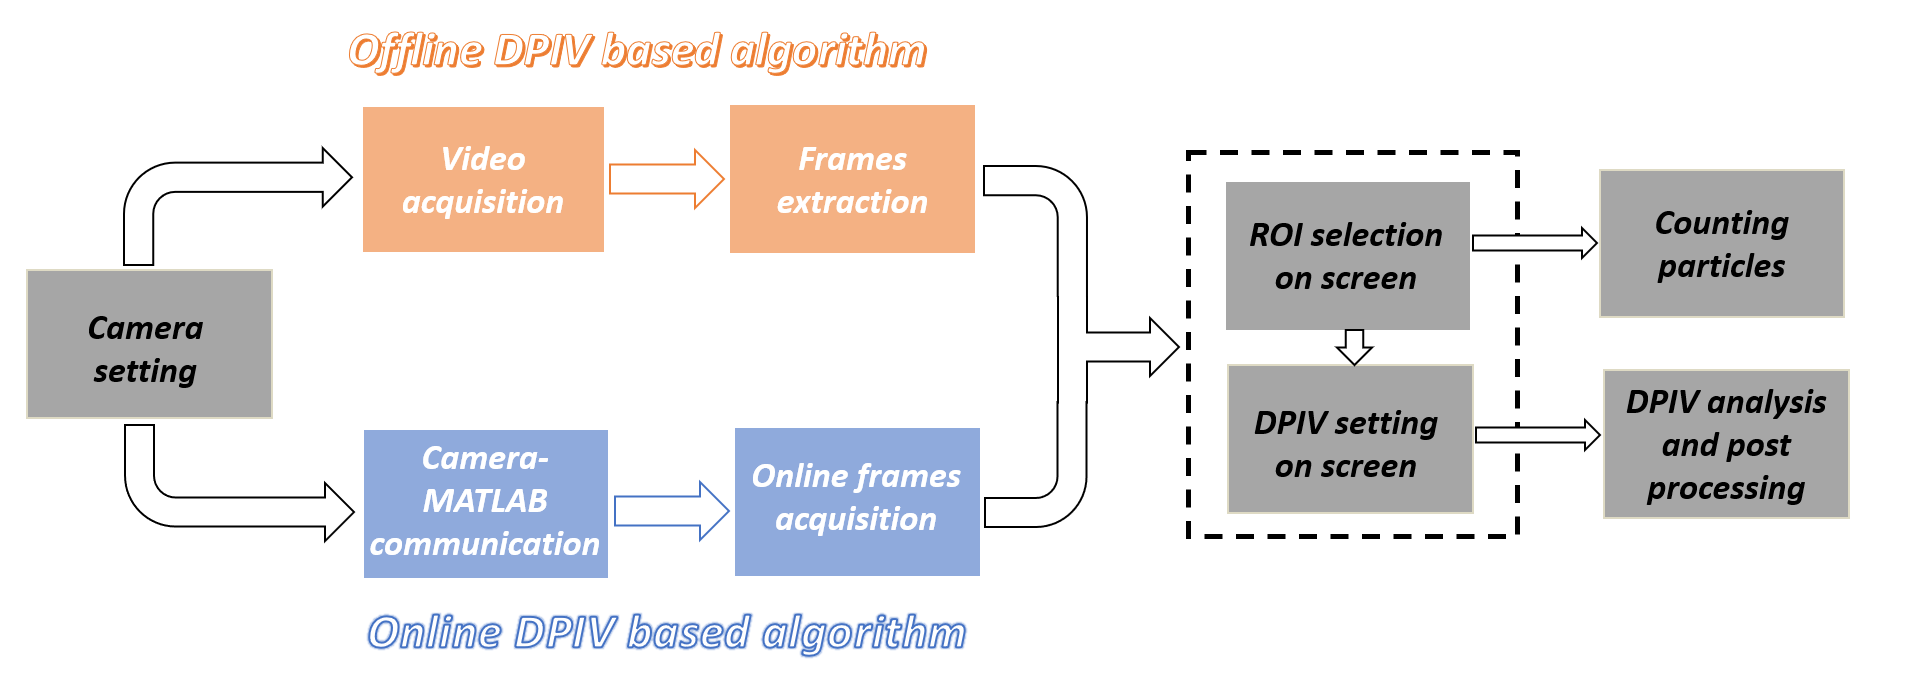
\includegraphics[width=2\columnwidth]{images/Algorithms}
	\centering{\caption{\label{Algorithms}DPIV-based offline and online algorithm implementation.}}
\end{figure*}

\begin{figure}[t]
	\centering
	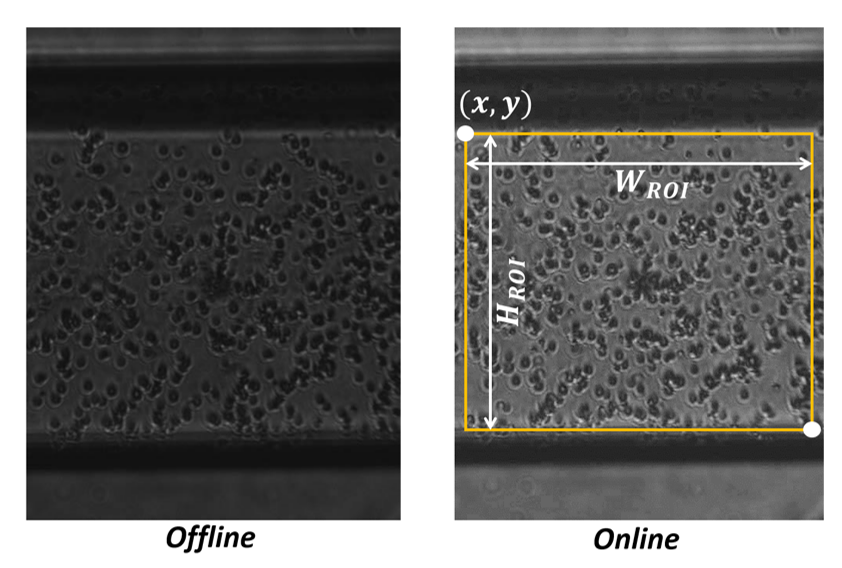
\includegraphics[width=1\columnwidth]{images/frames}
	\centering{\caption{\label{frame} Offline and online frame in comparison with the same camera parameters. ROI coordinates selection in the online frame. }}
\end{figure}

Both implementations share the initial steps of establishing the camera's settings (\fig\ref{Algorithms} block (1) \DS{no need to write "block (1)" just "(1)" is OK}) by making adjustments to the pixel size parameters listed in the camera datasheet, the magnification, the exposure time and the image gain. In particular, the latter is an amplification factor applied to all pixel values used for adjusting the pictures brightness level.
The online version differs significantly from the offline one due to the fact that the acquisition takes place in real time through a live stream from the CCD camera to the personal computer.  (\fig\ref{Algorithms} block (4)). This allows to capture process frames directly from the MATLAB routine and they are ready to be used for the analysis (\fig\ref{Algorithms} block (5)){We said to be quite general at this stage. So MATLAB for the moment shouldn't be mentioned}. The offline version, on the other hand, provides for a further step of uploading on MATLAB the video previously acquired through a dedicated software (\fig\ref{Algorithms} block (2)) and unpack it into the corresponding frames (\fig\ref{Algorithms} block (3)). 
Online frames acquisition through MATLAB allows to obtain a higher resolution process frame for the same camera parameters as it is shown in ~\fig\ref{frame}\DS{OK ---- to be verified}.
Having the data available, the algorithm proceeds in a similar way in the two implementations. 
An on-screen Region of Interest (ROI) selection procedure (\fig\ref{Algorithms} block (6)) allows setting the left-top corner of the image as the starting pixel and the right-down corner of the image as the end pixel. The resulting coordinates for the selection of the ROI are represented in ~\fig\ref{frame}: the abscissa ($\abscissa$) and ordinate ($\ordinate$) of the left-top point and the width ($\width$) and height ($\height$) of the region itself, obtained from the selection of the right-down point.\DS{The ROI choice is important but not at the point we use 9 rows to descibe its choice.} 
A DPIV analysis followed by a counting particles procedure are at this point carried out for the predefined interrogation ROIs. 
The first analysis concerns a DPIV-based algorithm (\fig\ref{Algorithms} block (8)) that provides instantaneous velocity measurements and visualization. Briefly summarizing the DPIV approach presented in ... \MANU{Add reference},it consists of a first collection of the time-varying velocity vector maps through the evaluation of the cross-correlation between ROIs of consecutive pairs of images. 
The velocity spatial distribution along the horizontal $\spatialmean{x}{i}{j}$ and vertical $\spatialmean{y}{i}{j}$ directions is obtained for each pairs of frames. A post processing procedure in terms of spatial average is done so that a single velocity value is obtained for each map. By repeating this for all the frames, two signals representing the trends of the average velocity over time are given, respectively $\mean{x}$ and $\mean{y}$.
The preliminary step of DPIV setting (\fig\ref{Algorithms} block (7)) concerns the possibility of opting for a multi-pass discrete Fourier transform (DFT) for the DPIV analysis, by setting the number of passes from 1 to 4, the corresponding interrogation areas and the step size.
A multi-pass DFT in frequency domain, as implemtend by the PIVlab tool\DS{Again, let's keep the generality of the discussion}, could be used in order to increase the accuracy. In the experimental campaign, detailed in \sect\ref{sec:setup}, the analysis was conducted by a three-passes DFT, reaching a good compromise between the resolution and the computational time. The three interrogation areas in pixels were chosen as follows: $Area1=64$, $Area2=32$ and $Area3=16$. The step size was set equal to the half of the last interrogation area ($Area3=16$), resulting in a value equal to 8 $\pixel$.
The micro-particles hydrodynamic response in time domain was evaluated by computing the range of the velocity signal $\meann$ in the two components $\abscissa$ and $\ordinate$, according to 
\begin{equation}
	\label{eqn:range}
	Range\meann=max(\meann)-min(\meann)
\end{equation}
The micro-particles hydrodynamic response in frequency domain was evaluated by computing the spectrum of $\meann$ in the two components $\abscissa$ and $\ordinate$. This provides informations on the frequency components involved in the dynamic process in terms of fundamental frequency, imposed by the hydrodynamic input and to investigate possible high-frequency components to be associated with intrinsic micro-particles behaviors.
\\The second analysis that this platform provides is the counting particles one (\fig\ref{Algorithms} block (9)). This procedure is based on highlighting the particles in the image distinguishing them from the background. It provides a continuous counting in the time of the micro-particles number in the investigated area, avoiding any manual and individual selecting of the frames to be studied \DS{Although current approaches rely on manual counting or others, (add references if any) the provided implementation makes use of a counting algorithm ...}. It allows to analyze the video frame by frame, count the number of particles and collect this information in a signal. This last can also be averaged over time to obtain a single average particles number for a given experimental condition.
\\The counting procedure is essential not only to have an idea of the number of micro-particles involved in the process, but, even more, when we want to compare the results obtained with different types of particles. The velocity obtained by the DPIV-based algorithm, in fact, can be strongly influenced by the number of particles present in the ROI since a spatial average is considered. It should also be considered that different micro-particles correspond to different densities which influence the number of them in the process. According to what has been said, it is necessary to normalize the velocity signals for the average particles number when we wants to compare processes characterized by micro-particles of different nature and physical properties.
\\Having selected the ROI, the counting operation follows some steps all based on image processing as presented in \MANU{Add reference}. A first conversion of the selected image portion to greyscale is followed by a duplication of the image. A Gaussian filter is applied and the resulting filtered image is subtracted from the greyscale one. A binarization procedure of the resulting image is performed.
At this point a function takes as input the binary image. It traces the exterior boundaries of particles and gives the number of them found.
Important parameters to be set are the minimum and maximum dimensions of the searched object in $\pixel$, in order to count among the found micro-particles only those that have an appropriate size. A threshold value based on the shape of the object should also be set. It defines the circularity of the object with a reference value equal to 1 that indicates a perfect circle.
Having defined all the parameters, the exterior boundaries of micro-particles are traced and the number of them is found for each frame.

\subsection{Experimental Setup and Campaigns}\label{sec:setup}

The experimental set-up is composed of a syringe pump, a microfluidic chip, an opto-mechanical system and a personal computer. A representation of it is reported in ~\fig\ref{setup}. Syringe pumps (neMESYS low-pressure module, Cetoni GmbH,
Korbussen, Germany) were used to inject the sample of particles or cells suspended in a fluid in the Y-junction squared rectilinear micro-channel (SMS0104, Thinxxs, Zweibrucken, Germany), 16~$[\rm mm]$ long and with a diameter of 320~$[\rm\mu m]$ (see ~\fig\ref{Platform}).


A CCD camera (340M Fast Frame, Thorlabs, Newton, NJ, USA) with a resolution of $640 \times 480$ \pixel (pixel size of 7.4~$[\rm\mu m]$, square) was included in the optomechanical system ((OTKB/M) Modular Optical Tweezers, Thorlabs, Newton, NJ, USA). Visible light from the LED source illuminates the sample and is then imaged on the CCD camera.
The CCD camera was connected through a USB connection with a PC for the data acquisition and the subsequent analysis phase in the dedicated software platform.


\begin{figure*}[t]
	\centering
	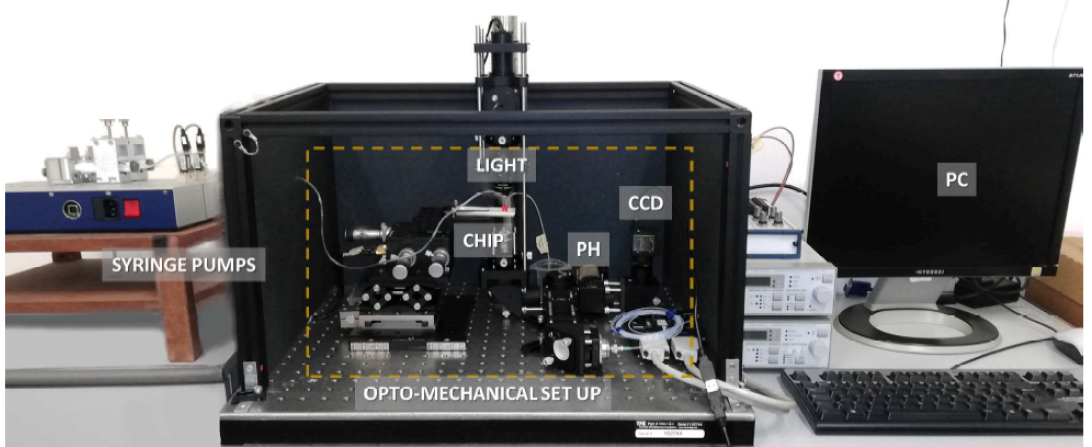
\includegraphics[width=2\columnwidth]{images/setup}
	\centering{\caption{\label{setup}A picture showing the experimental set-up.}}
\end{figure*}

A magnification of 10X (PLN, Olympus, Tokyo, Japan) has been used to scale up the channel images to be able to see more detail and increasing resolution.
Acquisitions and analyzes were performed using a SAMSUNG Galaxy Book PC, with an Intel Core i7 processor, INTEL Iris Xe Graphics, 16 GB RAM and 512 GB SSD.
\\The fluids employed for the experiments were obtained by diluting micro-particles in different solutions. The micro-particles were of two types: cells of eukaryotic origins with a diameter of 5 $[\rm\mu m]$ and artificial silica beads with a diameter of 6 $[\rm\mu m]$. Two types of particles have been used to investigate and compare the different behaviors of cells and synthetic particles. Their physical properties, such as mass, radius, volume and density, are summerized in ~\tab\ref{properties}. Two different types of yeast cell living conditions have been examined. In particular viable cells and exposed to cell death stimuli with hydrogen peroxide ($H_2O_2$).
Yeast cells were diluted in a saline solution, the phospate buffered saline (PBS, density of 1072 $\density$). By contrast, Silica beads micro-particles were diluted in two different solutions. A first one (density of 1200 $\density$) obtained by combining 20\% of water with 80\% of glycerol to avoid the deposition of the particles at the bottom of the channel thanks to the increment of the fluid density. The second solution is represented by PBS.
The microfluidic chip was fed with fluid on which an oscillating flow was imposed.
At the beginning a PBS flow and then a glycerol-water flow, without micro-particles suspendend on it, was recorded to quantify the effect of the fluid backgroung in the images. It was injected through syringe pumps with an external oscillating pressure at a frequency of $\frequency=0.1~\hertz$ and an amplitude of $\amplitude=0.1~\flow$.
\\The other 30 experiments that have been carried out are summarized in ~\tab\ref{offlineexp} and ~\tab\ref{onlineexp}, distinguished according to the software implementation used to analyze them (offline or online). Experiments with viable yeast cells and beads in glycerol-water solution were performed twice, to compare the results obtained with the two different implementations and test their consistency.
For all categories of cells and particles, the sample of fluid was fed into the micro-channel using an oscillating flow at a fixed frequency of $\frequency=0.1~\hertz$ and five different amplitude values $\amplitude\in~{0.05, 0.07, 0.1, 0.15, 0.2~\flow}$.


% Please add the following required packages to your document preamble:
% \usepackage{booktabs}
\begin{table}[t]
	\begin{tabular}{@{}lcccc@{}}
		\toprule
		\multicolumn{1}{c}{\textbf{Micro-particles}} & \textbf{\begin{tabular}[c]{@{}c@{}}Mass\\ {[}$Kg${]}\end{tabular}} & \textbf{\begin{tabular}[c]{@{}c@{}}Radius\\ {[}$m${]}\end{tabular}} & \textbf{\begin{tabular}[c]{@{}c@{}}Volume\\ {[}$m^3${]}\end{tabular}} & \textbf{\begin{tabular}[c]{@{}c@{}}Density\\ {[}$Kg/m^3${]}\end{tabular}} \\ \midrule
		\textit{Yeast cells}                         & 7.37 $e^{-14}$                                      & 2.5 $e^{-6}$                                       & 6.54 $e^{-17}$                                                          & 1126                                                                                     \\
		\textit{Silica beads}                        & 1.36 $e^{-13}$                                      & 3.0 $e^{-6}$                                         & 1.13 $e^{-16}$                                                         & 1200                                                                                     \\ \bottomrule
	\end{tabular}
\centering{\caption{\label{properties}Physical properties of micro-particles.}}
\end{table}


\begin{table}[t]
	\begin{tabular}{@{}lp{0.85cm}c@{}}
		\toprule
		\rowcolor[HTML]{FFFFFF} 
		\textbf{Micro-particles}                            & \textbf{\begin{tabular}[c]{@{}c@{}}Frequency \\ $f_i$ {[}$Hz${]}\end{tabular}} & \textbf{\begin{tabular}[c]{@{}c@{}}Amplitude \\ $A$\,{[}\,$ml/min${]}\end{tabular}} \\ \midrule
		\textit{Viable Yeast cells}                        & 0.1                                                                       & 0.05, 0.07, 0.1, 015, 0.2                                                                                               \\
		\textit{Yeast cells exposed to cell death stimuli} & 0.1                                                                       & 0.05, 0.07, 0.1, 015, 0.2                                                                                               \\
		\textit{Beads in PBS}                              & 0.1                                                                       & 0.05, 0.07, 0.1, 015, 0.2                                                                                               \\
		\textit{Beads in glycerol-water}                   & 0.1                                                                       & 0.05, 0.07, 0.1, 015, 0.2                                                                                               \\ \bottomrule
	\end{tabular}
\centering{\caption{\label{offlineexp}Offline experimetal campaign.}}
\end{table}

\begin{table}[t!]
	\begin{tabular}{@{}lcc@{}}
		\toprule
		\rowcolor[HTML]{FFFFFF} 
		\textbf{Micro-particles}          & \textbf{\begin{tabular}[c]{@{}c@{}}Frequency \\ $f_i$ {[}$Hz${]}\end{tabular}} & \textbf{\begin{tabular}[c]{@{}c@{}}Amplitude \\ $A$\,{[}\,$ml/min${]}\end{tabular}} \\ \midrule
		\textit{Viable Yeast cells}    
		     & 0.1                                                                       & 0.05, 0.07, 0.1, 015, 0.2                                                   \\
		\textit{Beads in glycerol-water} & 0.1                                                                       & 0.05, 0.07, 0.1, 015, 0.2                                                   \\ \bottomrule
	\end{tabular}
\centering{\caption{\label{onlineexp}Online experimetal campaign.}}
\end{table}

\begin{table}[t!]
	\begin{tabular}{@{}lcccc@{}}
		\toprule
		\multicolumn{5}{c}{\textbf{Region of Interest (ROI)}}                                                                                         \\ \midrule
		& \textbf{$x$} & \textbf{$y$} & \textbf{$H_{ROI}$} & \textbf{$W_{ROI}$} \\
		\textit{Yeast cells}  & 6          & 131        & 473                                          & 360                                          \\
		\textit{Silica beads} & 7          & 67         & 467                                          & 411                                          \\ \bottomrule
	\end{tabular}
	\centering{\caption{\label{roi}ROI coordinates set for the image area acquired and analyzed in the performed experiments. }}
\end{table}

The data were recorded considering different time intervals in the two types of algorithms:
\begin{itemize}
	\item \textit{Offline algorithm}: data recorded for 60 $\seconds$, with a video frame rate of 57 $\framerate$, around 3420 frames per experiment.
	\item \textit{Online algorithm}: data recorded for 15 $\seconds$, with a video frame rate of 57 $\framerate$, around 855 frames per experiment. 
\end{itemize}

In the online implementation, in particular, the acquisition took place through the communication between the CCD camera and MATLAB, downloading the \textit{Windows SDK and Doc. for Scientific Cameras}.
The image gain was set equal to 200 and the exposure time equal to 17000 $[\rm\mu s]$, resulting in a framerate of 57 $\framerate$. The pixelsize value set at 7.4~$[\rm\mu m]$ was obtained from the camera datasheet.
Another important step to perform before the start of the DPIV and
counting particles analysis is the selection of the ROI.
It was determined as described in \sect\ref{sec:method} and the coordinates are reported in ~\tab\ref{roi}. 
\\Having selected the investigated area, the setting of the parameters for the multi-pass DFT for the DPIV analysis was done as described in \sect\ref{sec:method}. Following, some details on the choice of the parameters for the counting particles analysis are reported. For the yeast cells and the silica beads the minimum area was set to 1 $\apixel$ and the maximum was set to 2 $\pixel$. Due to the circular geometry of micro-particles, the threshold was set equal to 1 that indicates a perfect circle.

\section{Results and discussion}
In this chapter the experimental results are presented. In particular in \sect\ref{sec:suspended-particles} we will discuss the behavior of synthetic particles related to the fluid in which they are suspended and in \sect\ref{sec:comparison} we will compare the hydrodynamic response of the different types of cells, viable and dead, and synthetic particles. Referring to the methodology as you did if you like. \sect\ref{sec:OnlineOffline} shows a comparison of the results obtained with the two implementations.
Since the micro-particles are induced to move in the horizontal direction, this will be the velocity component considered in the subsequent analysis. 
%Looking at the movement of the micro-particles along the micro-channel and considering also the image orientation, the dominant velocity component is the horizonatal one. In fact, the trend of the horizontal velocity component $<V_x(t)>$ shows the periodicity of the oscillating input flow imposed. This component is the one taken in consideration for the following analysis. 


\subsection{Particles suspended in fluids with different densities}\label{sec:suspended-particles}

The described algorithm was used to study how the hydrodynamic response of synthetic micro particles, silica beads, can be related to their physical properties and differ according to the fluid in which they are suspended. To compare the results obtained for the same kind of particles suspended in different fluids, the velocity signal $\mean{x}$ was computed per each experiment, by the DPIV-based algorithm described in \sect\ref{sec:method}.

\begin{figure}[t]
\centering
    \begin{subfigure}[b]{\columnwidth}
    \centering
	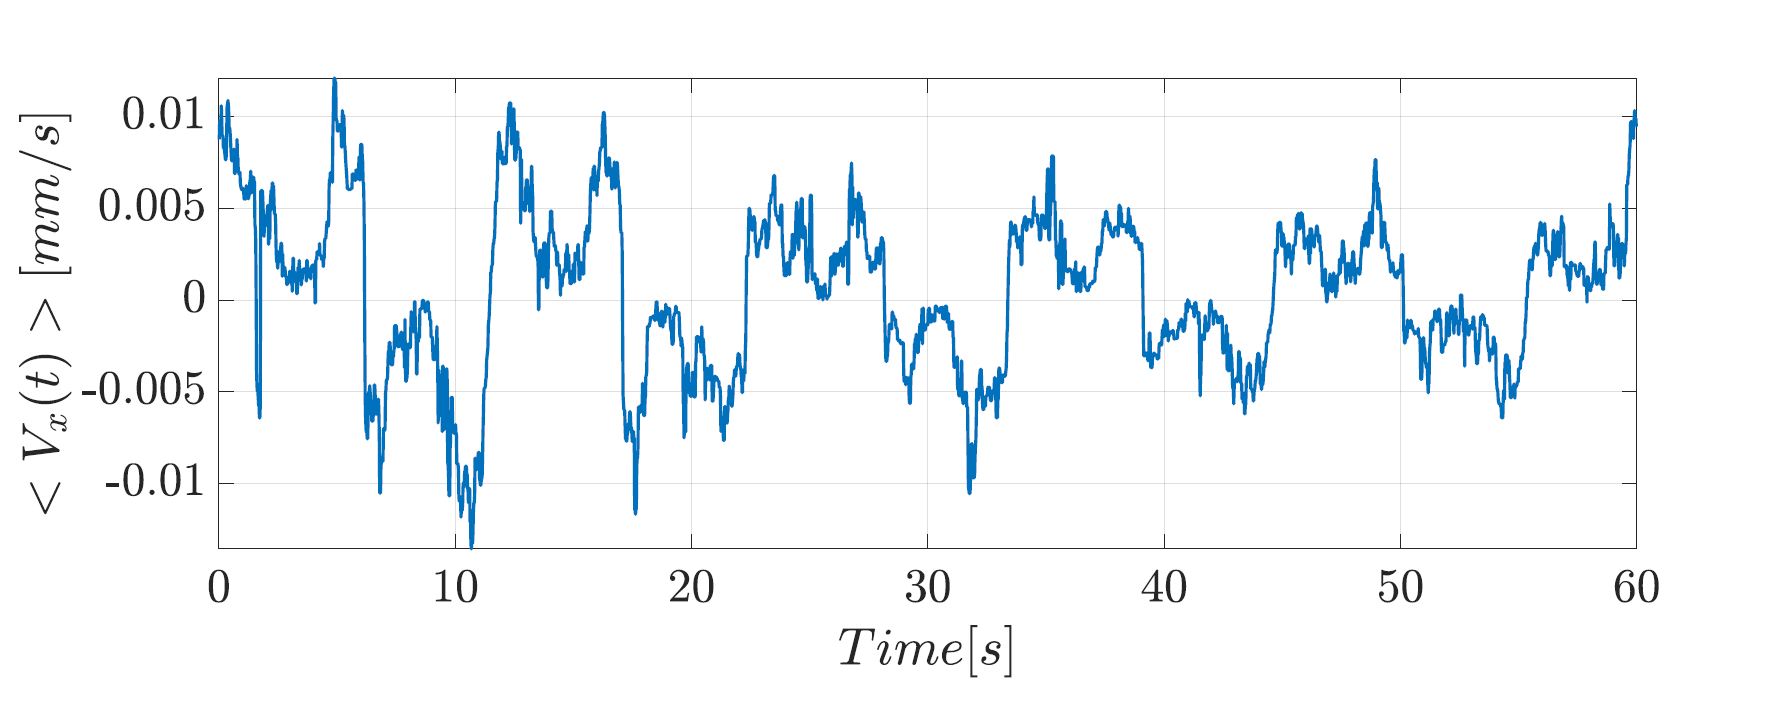
\includegraphics[width=1\columnwidth]{images/BeadsA}
	\caption{}
	\label{A}
    \end{subfigure}
    \begin{subfigure}[b]{\columnwidth}
	\centering
	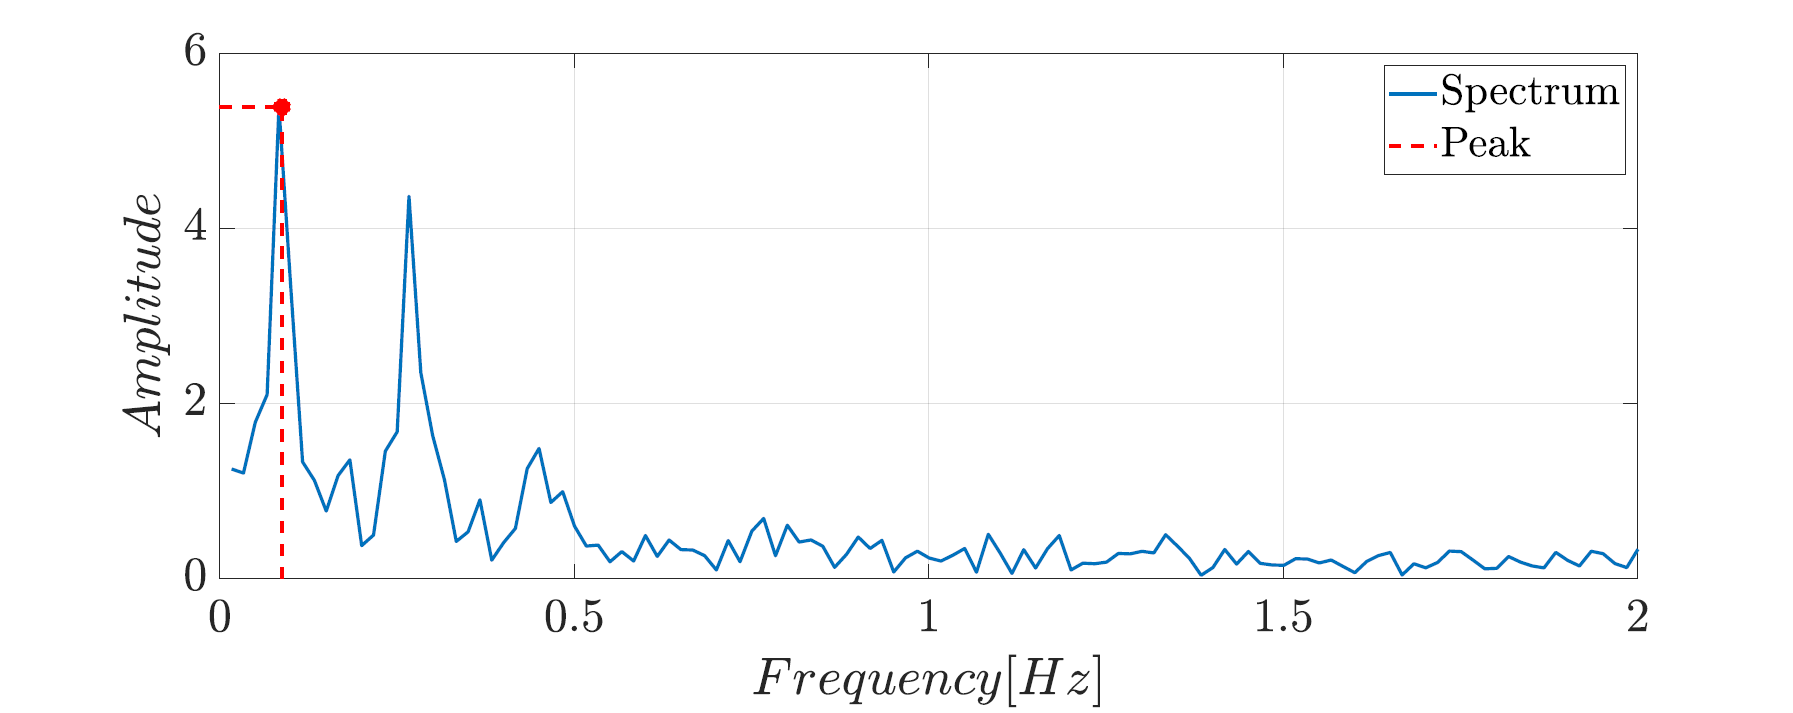
\includegraphics[width=1\columnwidth]{images/BeadsB}
	\caption{}
	\label{B}
    \end{subfigure}
    \begin{subfigure}[b]{\columnwidth}
	\centering
	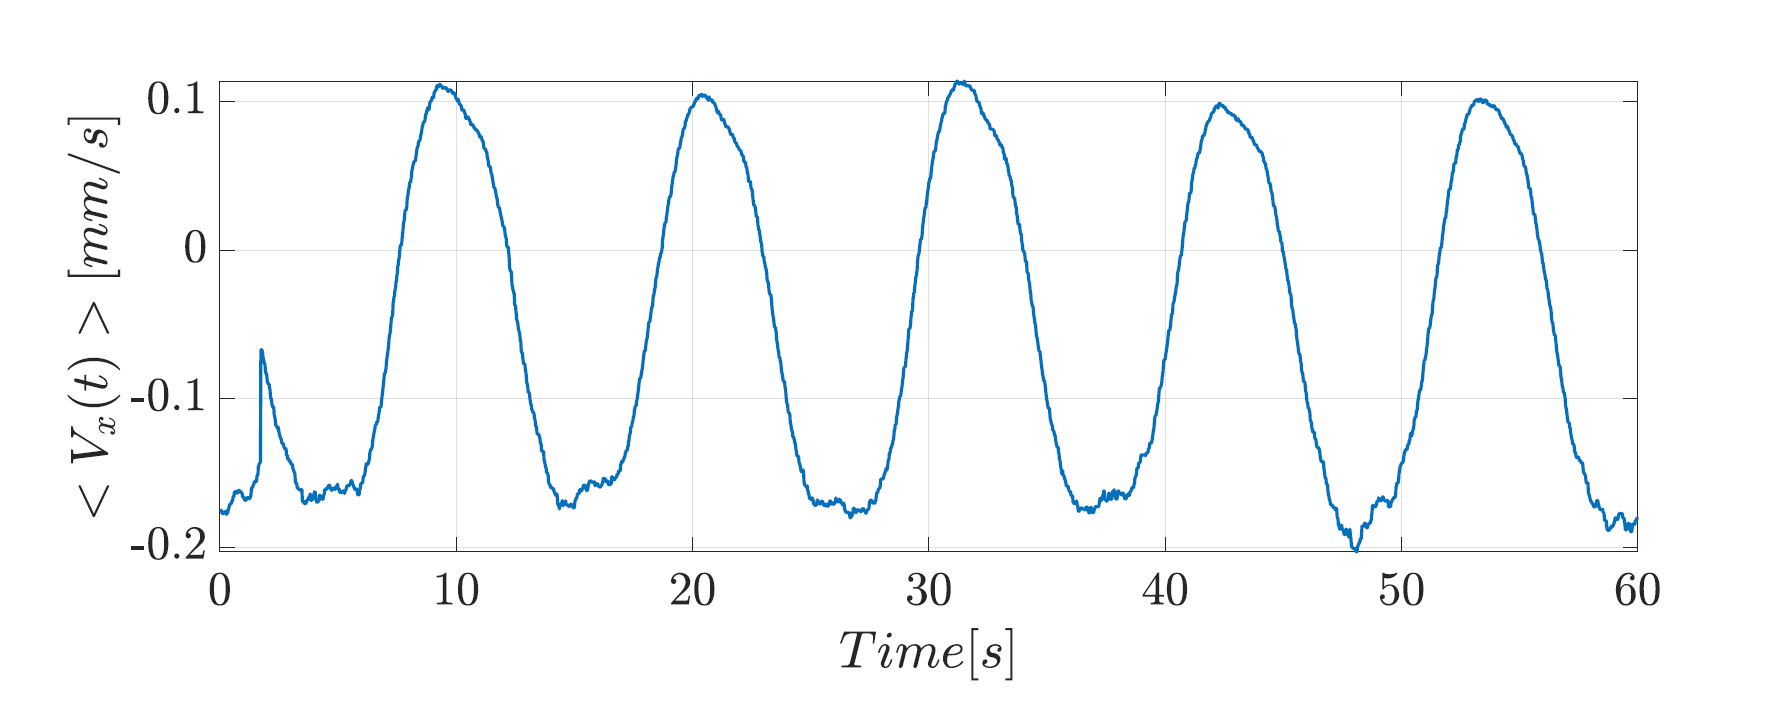
\includegraphics[width=1\columnwidth]{images/BeadsC}
	\caption{}
	\label{C}
    \end{subfigure}
    \begin{subfigure}[b]{\columnwidth}
	\centering
	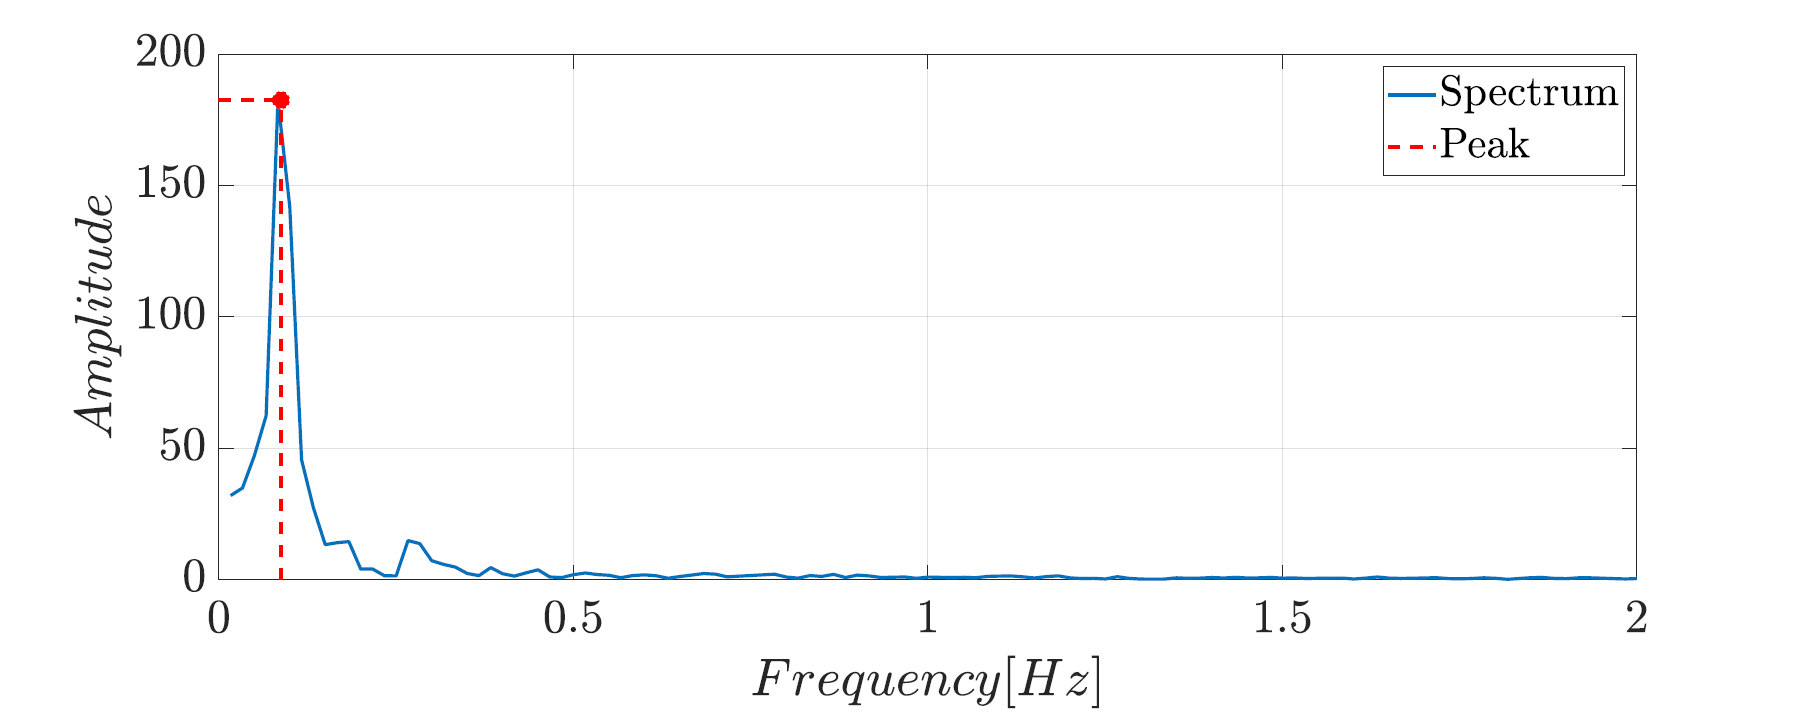
\includegraphics[width=1\columnwidth]{images/BeadsD}
	\caption{}
	\label{D}
    \end{subfigure}
\centering{\caption{\label{Beads}The velocity trends $\mean{x}$ and its spectrum obtained in the experimental condition with $\amplitude=0.1~\flow$ and  $\frequency=0.1~\hertz$: velocity signal (a) and its spectrum (b) of silica beads in PBS solution and velocity signal (c) and its spectrum (d) of silica beads in glycerol-water solution.}}
\end{figure} 

\begin{figure*}[t]
	\centering
	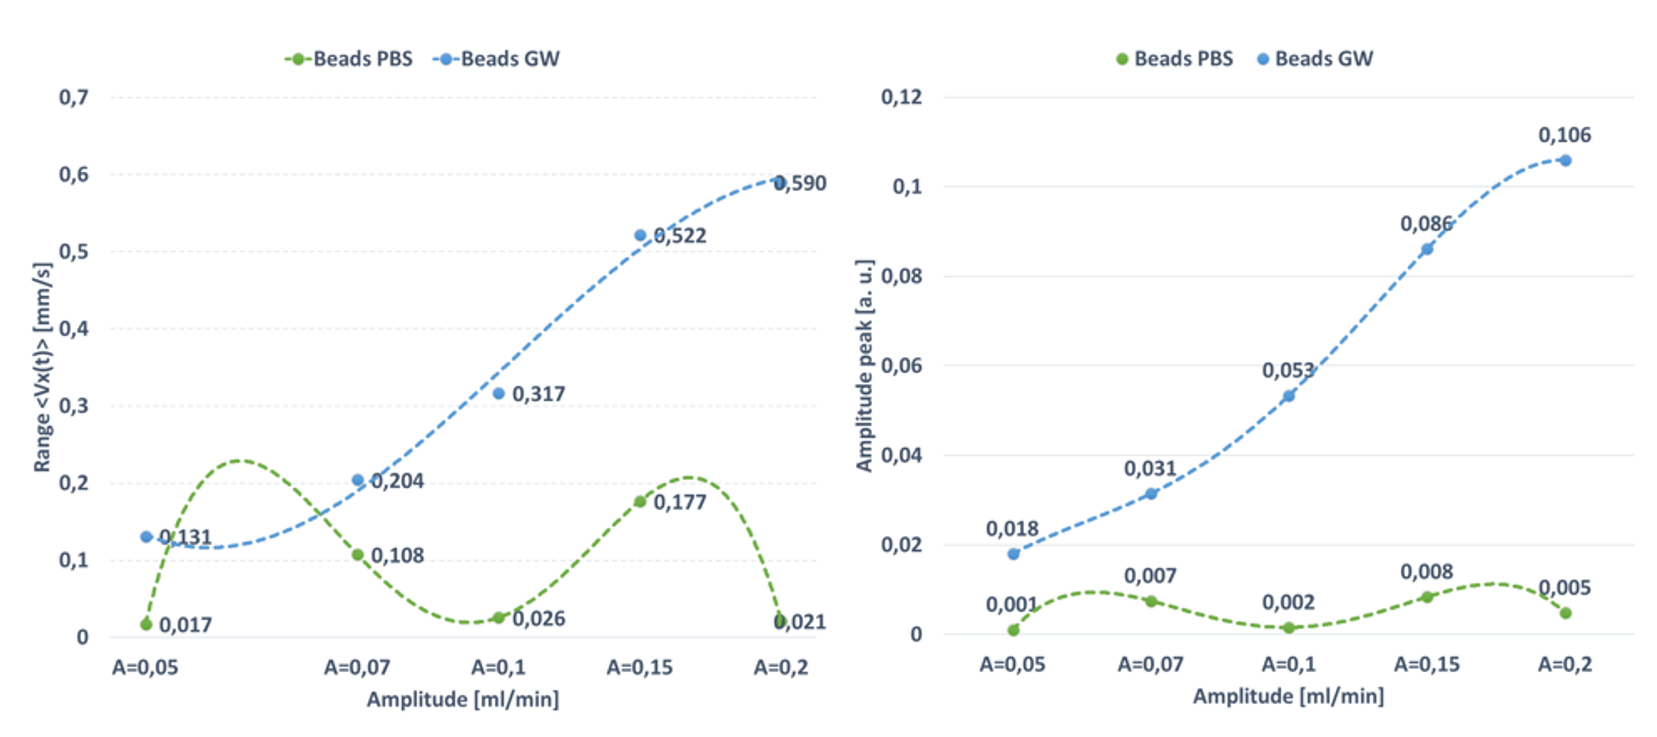
\includegraphics[width=2\columnwidth]{images/BeadsFinal}
	\centering{\caption{\label{BeadsFinal}Parameters $\range$ and $\peak$ at the fundamental frequency varying the oscillating input flow strength at the inlet $\amplitude$ at $\frequency=0.1~\hertz$ for silica beads in PBS and glycerol-water (GW) solution.}}
\end{figure*}

In ~\fig\ref{Beads}, for silica beads in PBS and in glycerol-water solution, in the experimental condition with $\amplitude=0.1~\flow$ and  $\frequency=0.1~\hertz$, the velocity signals in the dominant component  $<V_x(t)>$ and their spectrum are plotted.
It can be noted that the speed signal relating to the silica beads sample in the PBS solution (see ~\fig\ref{Beads}(a)) is noisier than the speed signal relating to the silica beads sample in the glycerol-water solution (see ~\fig\ref{Beads}(c)). This is given by the fact that since the silica beads have a higher density than PBS, they tend to settle in the bottom of the micro channel, putting up resistance to the imposed hydrodynamic actuation at the input. Suspended beads in a solution of the same density have shown to be an effective solution to this problem. This allows beads to float in the fluid and not to pose resistance to the hydrodynamic input that is imposed. The speed signal relating to the silica beads sample in the glycerol-water solution (see ~\fig\ref{Beads}(c)) shows a shape similar to that expected from the input flux supplied, a sine wave with frequency $\frequency=0.1~\hertz$, detected from the fundamental frequency in the spectrum, and amplitude $\amplitude=0.1~\flow$.
\\The micro-particles hydrodynamic response in time domain was evaluated by computing the range of the velocity signal $\mean{x}$, as shown in \eqn (\ref{eqn:range}). ~\fig\ref{BeadsFinal} shows the value of $\range$ and the amplitude peak at the fundamental frequency, $\peak$, for each experimental condition. The two curves are related to silica beads in the two different solutions considered and each point of the curves is correlated to the amplitude of the external oscillating input flow strength $\amplitude$ with a constant $\frequency=0.1~\hertz$. 
\\The curve related to the beads in PBS does not show any correlation between the imposed input and the hydrodynamic response of the micro-particles. The curve relating to the beads in the glycerol-water solution shows how the parameters examined in the time domain and in the frequency domain increase as the input amplitude increases, showing a correlation between the input and the hydrodynamic response of the micro-particles.
Since silica beads are synthetic particles, what we expect is that they do not provide any resistance to the input sources and so the glycerol solution is the most suitable among the analyzed ones because it allows to show up this behavior.
For this reason, in \sect\ref{sec:comparison} in which the comparison between synthetic particles, live cells and cells exposed to death stimuli is made, and in \sect\ref{sec:OnlineOffline} in which the results obtained from the online and offline platform are compared, only the results relating to silica beads in the glycerol-water solution will be considered beacause they allowed a better process characterization.

\subsection{Viable cells, Dead cells and Synthetic Particles in comparison}\label{sec:comparison}

The DPIV-based and micro-particles counting algorithms were used to analyze the data collected in the experimental campaigns related to yeast cells in different living conditions. This allowed to investigate how the hydrodynamic response of cells could be correlated to their living condition.  To compare the results obtained for different kind of cells' living condition, the velocity signal $\mean{x}$ was computed by the DPIV-based algorithm described in \sect\ref{sec:method}, the spectrum of each signal was evaluated and the average number of micro-particles $\particles$ was computed for each experiment. 
In particular, the results relating to viable yeast cells and viable yeast cells exposed to cell death stimuli, induced by an apoptotic process of death, i.e. a mechanism of genetically programmed death, are reported \DS{TODO: provide additional details in the introduction about apoptosis and add references}. These two conditions allowed to correlate the hydrodynamic response of the micro-particles to their physical properties according to the different living conditions. This allowed a characterization of the same type of cells, the yeast cells, in the different phases of the cell cycle.

\begin{figure}[t]
	\centering
	\begin{subfigure}[b]{\columnwidth}
		\centering
		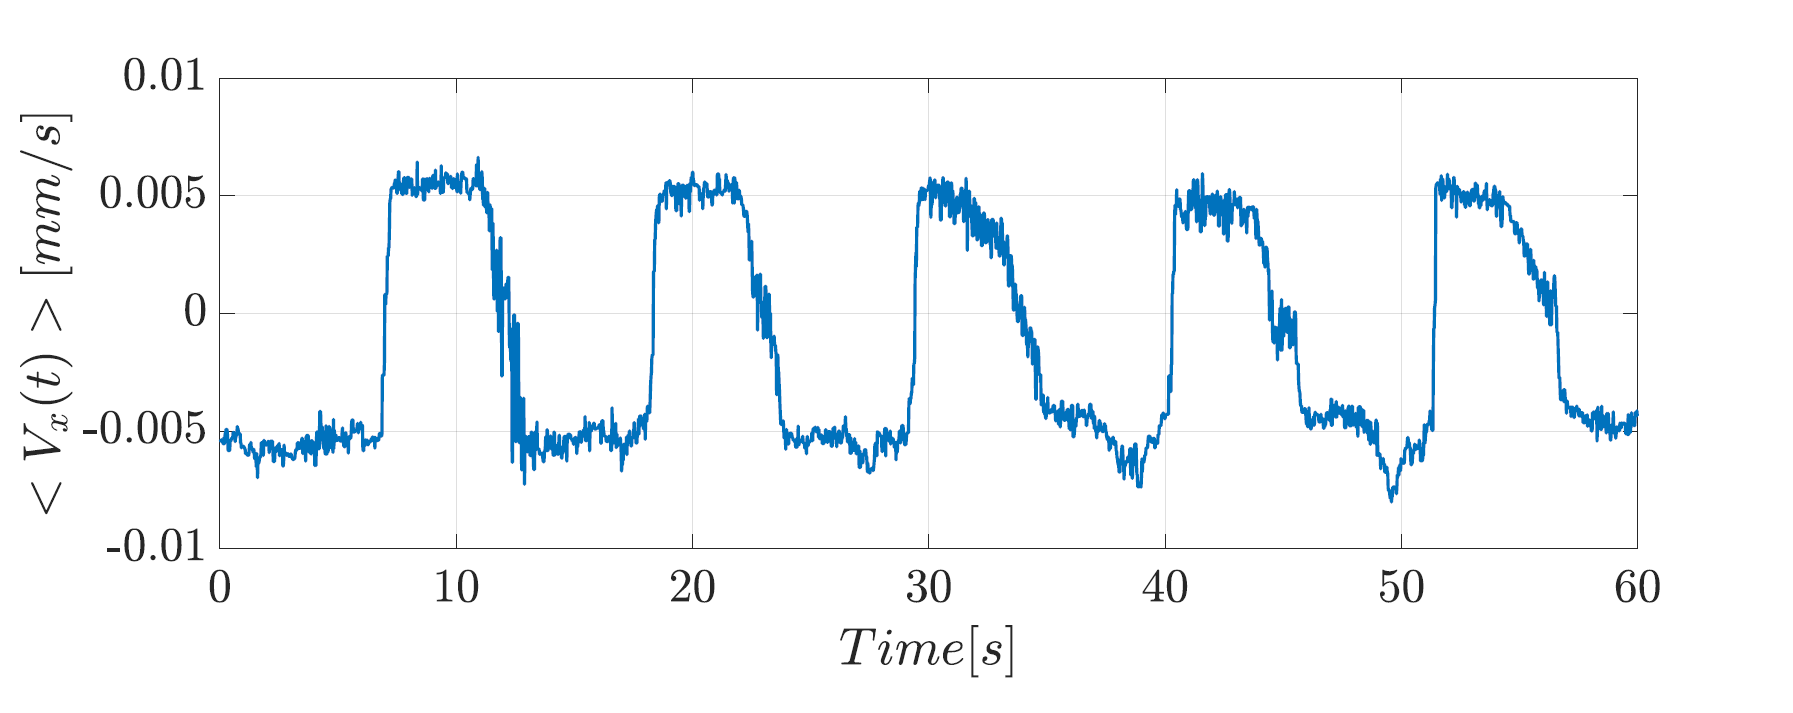
\includegraphics[width=1\columnwidth]{images/YeastA}
		\caption{}
		\label{A}
	\end{subfigure}
	\begin{subfigure}[b]{\columnwidth}
		\centering
		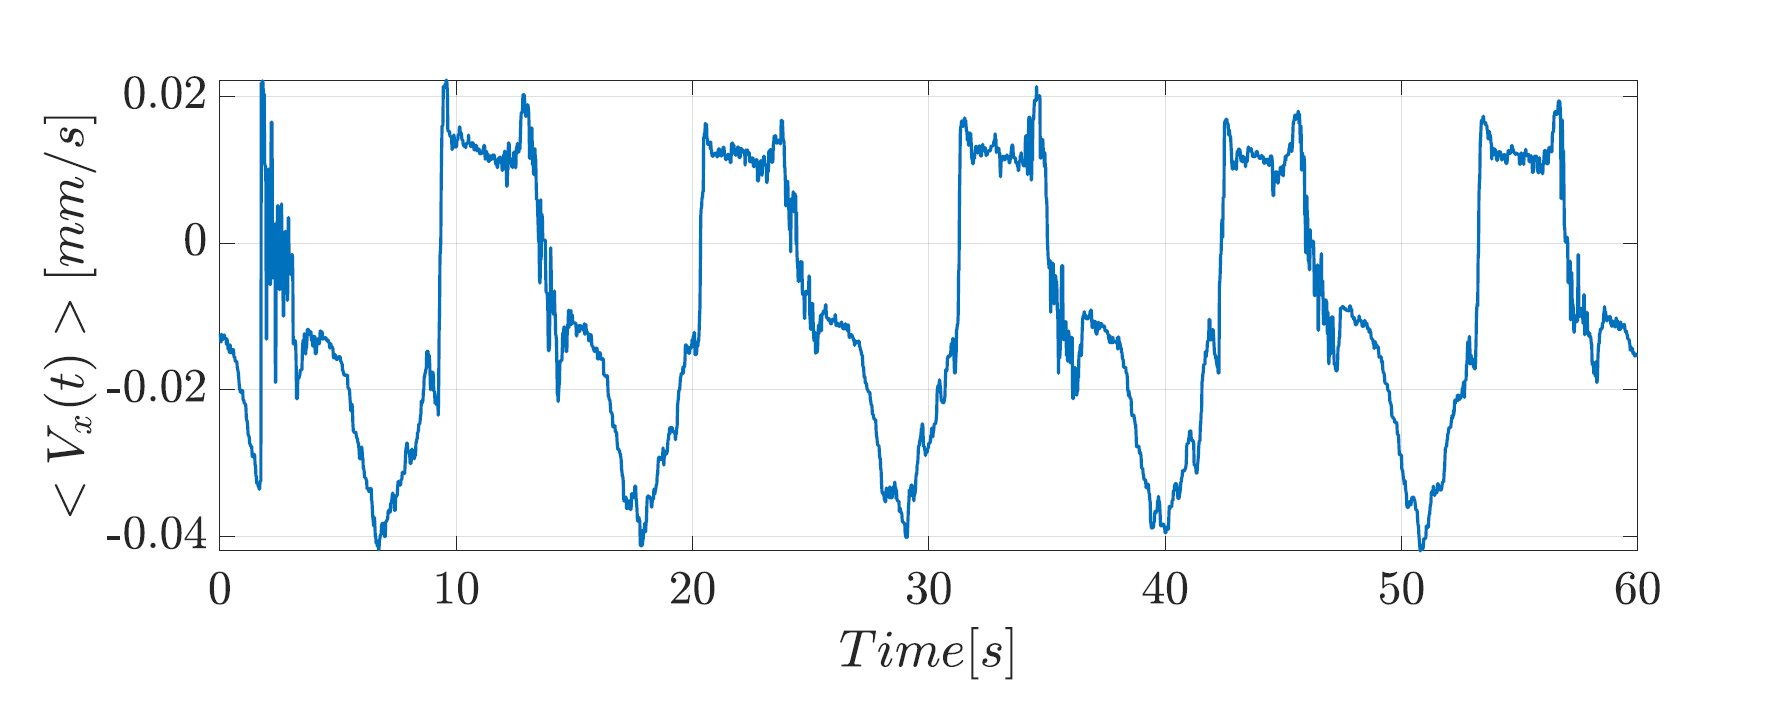
\includegraphics[width=1\columnwidth]{images/YeastB}
		\caption{}
		\label{B}
	\end{subfigure}
	\centering{\caption{\label{Yeast}The velocity trends $\mean{x}$ in the experimental condition with $\amplitude=0.1~\flow$ and  $\frequency=0.1~\hertz$: viable yeast cell (a) and yeast cell exposed to cell death stimuli (b).}}
\end{figure}  

In ~\fig\ref{Yeast}, for viable and exposed to cell death stimuli yeast cells, in the experimental condition with $\amplitude=0.1~\flow$ and  $\frequency=0.1~\hertz$, the velocity signals in the dominant component  $\mean{x}$ are plotted. The different oscillating trends of the velocity signals highlights the effects induced by the oscillating input flow in different cell living condition. In particular, considering the same experimental condition, the amplitude of the velocity trend for viable yeast cells (see ~\fig\ref{Yeast}(a)) is lower than the one found for yeast cells exposed to cell death stimuli. 
In the condition of viable yeast cells there is a greater resistance from the cells to the force imposed on the input, resulting in a lower maximum speed value reached compared to that of yeast cells exposed to cell death stimuli.

\begin{figure}[t]
	\centering
	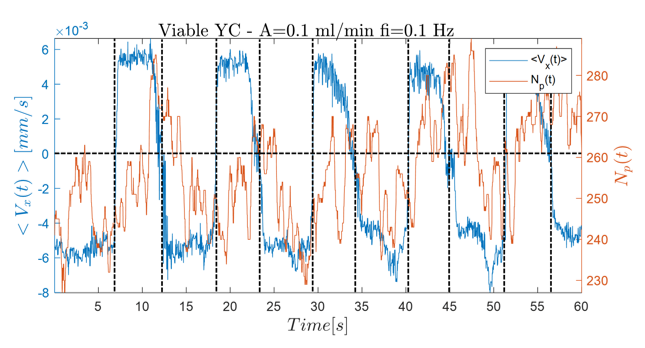
\includegraphics[width=1\columnwidth]{images/VelPar}
	\centering{\caption{\label{VelPar}The velocity trend $\mean{x}$ compared with the trend of $\particles$ in the experimental condition with viable yeast cells and $\amplitude=0.1~\flow$ and  $\frequency=0.1~\hertz$.}\MANU{Discuss with professor the possibility to choose another experimental condition in which the concept is more evident. After that modify the figure as done with the other.}}
\end{figure}

In ~\fig\ref{VelPar} the superposition of the trend of  $\mean{x}$ and the trend of $\particles$ is plotted, with viable yeast cells in the same experimental condition as before. In the instants in which the speed signal is 0 $\flow$, the signal of the trend of the particles assumes the maximum value; this is due to the fact that when the speed is zero, particles stop and accumulate.
\\In the instants in which the velocity signal is at the maximum or minimum value, the particle trend signal assumes the minimum value, because particles are in motion, in one direction or in the other, and the fewest number of them are counted by the algorithm. This is a consequence of the hydrodynamic stimulus imposed by the mechanical actuation through the syringe pumps flow rate, i.e. particles tend to be highly concentrated when the stimulus reaches the zero value, otherwise they are more dispersed during the rising phase of the stimulus, indipendently of its direction.

\begin{figure}[t]
	\centering
	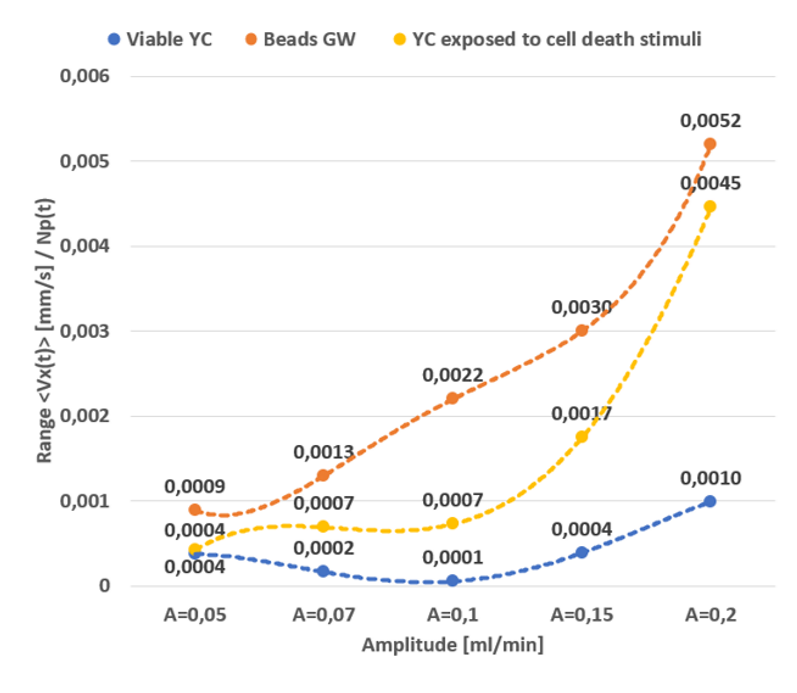
\includegraphics[width=1\columnwidth]{images/Comparison}
	\centering{\caption{\label{Comparison}The parameter ($Range<V_x(t)>$) varying the oscillating input flow strength at the inlet $A$ at a frequency $f_i= 0.1 Hz$: comparison between viable yeast cells, yeast cells exposed to cell death stimuli and silica beads in the glycerol-water (GW) solution. \MANU{Should we fit the points with a broken line instead of using a degree 4 polynomial?}}}
\end{figure}

~\fig\ref{Comparison} shows the value of $\range$ for each experimental condition. The three curves are related to viable yeast cells, yeast cells exposed to cell death stimuli and silica beads in the glycerol-water solution. Each point of the curves is correlated to the amplitude of the external oscillating input flow strength $\amplitude$ with a constant  $f_i= 0.1 Hz$. 
Because of the fact that micro-particles of different natures are being compared, a normalization of the $\range$ to the average number of particles was carried out. This procedure was applied due to the fact that the micro-particles density is different in each experimental condition and thanks to this normalization it is possible to compare the results obtained. 
\\The micro-particles hydrodynamic response comparison in time domain was evaluated by computing the range of the velocity signal $\mean{x}$, as shown in \eqn(\ref{eqn:range}) and normalizing it with respect to the average number of micro-particles $\particles$, computed in the investigated area following the procedure described in \sect\ref{sec:method}.
From ~\fig\ref{Comparison} it is possible to notice that, for all the experimental conditions, the curve relating to yeast cells exposed to cell death stimuli is always in the middle, between the one relating to viable yeast cells and the one relating to silica beads in the glycerol-water solution.
Yeast cells vary their behavior according to their different living conditions taking on characteristics more typical of synthetic particles, i.e. silica beads, when they are exposed to death stimuli. In fact, the results show that their behavior is comparable with particles of lower density and with the fluid on which they are suspended as they exhibit no resistance to the input flows while attaining higher velocities than the viable yeast cells.

\subsection{Online vs offline}\label{sec:OnlineOffline}
\DS{Before going into the details with this part and its revision, please, consider to make all the necessary steps to identify that the camera settings are not modified by Matlab. }
To test the consistency of the two DPIV-based implementations, a subset of the experiments was tested and analyzed also through the DPIV-based online implementation, detailed in ~\tab\ref{onlineexp}. Two categories of micro-particles were considered, more precisely viable yeast cells and silica beads in the glycerol-water solution. The sample of fluid was fed into the micro-channel using an oscillating flow at a fixed frequency of $\frequency=0.1~\hertz$ and five different amplitude values $\amplitude\in~{0.05, 0.07, 0.1, 0.15, 0.2~\flow}$.. Process frames were acquired for a time interval of 15 $\seconds$ for each experimental condition. 
The results obtained through the online implementation were compared with those obtained through the offline platform for the same micro-particle category and experimental conditions.

\begin{figure}[t]
	\centering
	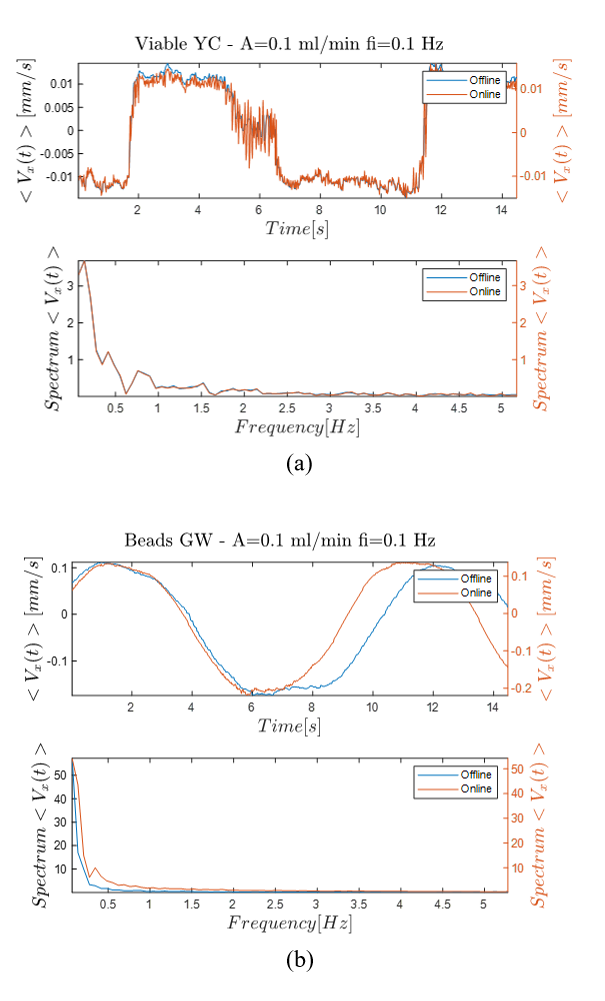
\includegraphics[width=1\columnwidth]{images/OnOff}
	\centering{\caption{\label{OnOff}Superimposition of the velocity trends $<V_x(t)>$ and its spectrum obtained in the experimental condition with {$A=0.1 ml/min, f_i= 0.1 Hz$} through online and offline platforms: (a) viable yeast cells and (b) silica beads in glycerol-water solution.\DS{Why at t=5-7 s, the online algorithm output is quite noisy in fig. 10 (a)? \DS{No need to have the labels on the right, since by using the legend labels "offline", "online", we are totally fine.} \DS{The legend shouldn't go over the signals.}\DS{No need to have the labels on the right, since by using the legend labels "offline", "online", we are totally fine.}\DS{The font should be bigger.}  }}}
\end{figure}

\begin{figure*}[t]
	\centering
	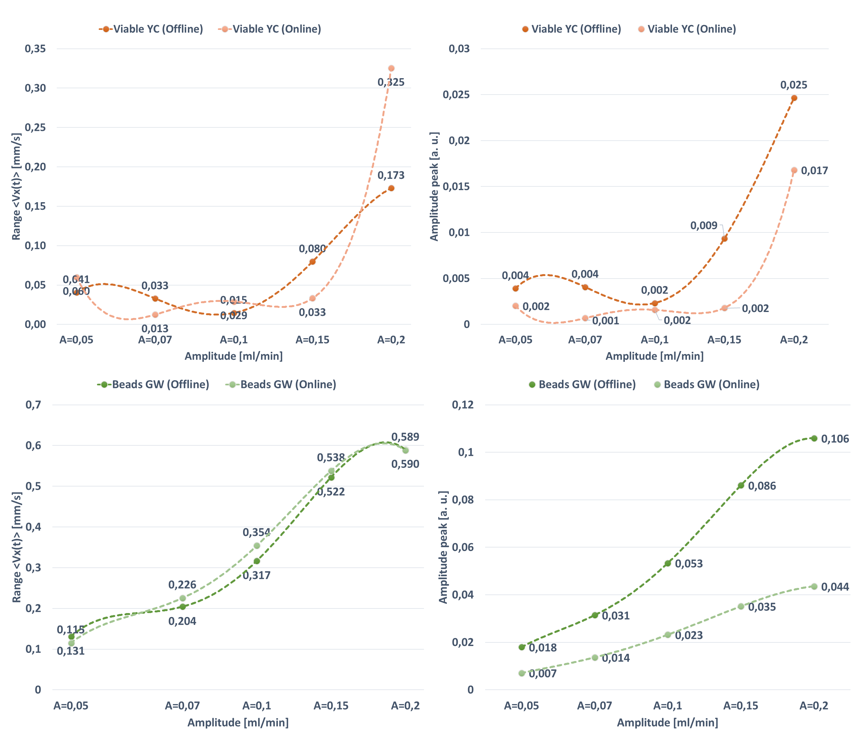
\includegraphics[width=2\columnwidth]{images/ComparisonOnOff}
	\centering{\caption{\label{ComparisonOnOff}Comparison of the parameter ($Range<V_x(t)>$) and the parameter ($Amplitude peak$) at the fundamental frequency varying the oscillating input flow strength at the inlet $A$ at a frequency $f_i= 0.1 Hz$ through online and offline platforms: (a) viable yeast cells and (b) silica beads in glycerol-water (GW) solution.}}
\end{figure*}

In ~\fig\ref{OnOff}, for viable yeast cells and silica beads in the glycerol-water solution, in the experimental condition with $\amplitude=0.1~\flow$ and  $\frequency=0.1~\hertz$, the superimposition of the velocity signals in the dominant component  $\mean{x}$ and of their spectrum are plotted.
From a first comparison it can be seen that the two curves are perfectly superimposable: the velocity values and the amplitude of the frequency peak are comparable in the two cases.
~\fig\ref{ComparisonOnOff} shows the value of the ($\range$) and the $\peak$) for the two experimental condition. The two plots are related to viable yeast cells and to silica beads in the glycerol-water solution in the online e offline case. Each point of the curves is correlated to the amplitude of the external oscillating input flow strength $\amplitude$ with a constant $\frequency=0.1~\hertz$. 
The comparison was made in the time and frequency domain and also in terms of statistical parameters, calculating the variations, indicated as $\Delta$, between two point of the curves correlated to the same amplitude of the external oscillating input flow strength $\amplitude$, the average among the various $\Delta$ values, the standard deviation and the coefficient of variation. This last is a dispersion index that allows to compare measurements of phenomena referred to different units of measurement, as it is a dimensionless quantity. 
\\It was calculated to establish which approach is more robust between the comparison in the time domain through the $\range$) or in the frequency domain through the $\peak$.
\\Being $\mu\neq0$ the arithmetic mean of a quantity and $\sigma$ its standard deviation, then the coefficient of variation is:

\begin{equation}
	\label{eqn:coefficient}
	\sigma^*=\frac{\sigma}{ \left|\mu\right|}
\end{equation}

\begin{figure}[t]
	\centering
	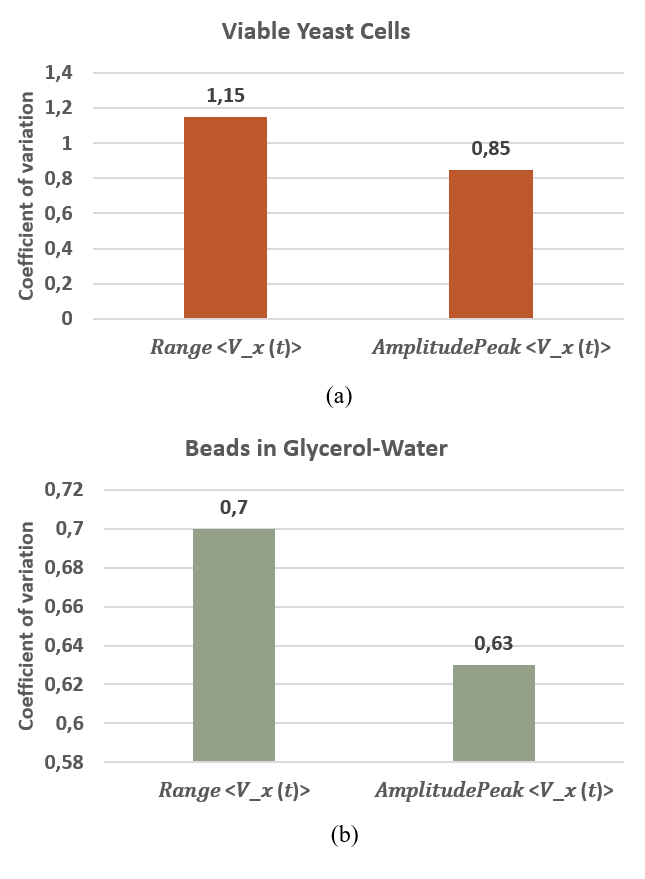
\includegraphics[width=1\columnwidth]{images/Coeff}
	\centering{\caption{\label{Coeff}Coefficient of variation evaluated from the $Range<V_x(t)>$ parameter and the $Amplitude peak$ parameter: (a) viable yeast cells and (b) silica beads in glycerol-water (GW) solution.}}
\end{figure}

The coefficient of variation is often compared between two or more groups to understand which group has a lower standard deviation relative to its mean. 
~\fig\ref{Coeff} shows a bar graph representing the value of the coefficients of variation calculated from the $\range$ parameter and the $\peak$ for both categories of micro-particles: viable yeast cells and silica beads in the glycerol-water solution. 
In both cases there is a smaller coefficient of variation calculated from the $\peak$ values. The frequency approach could be considered more robust because it is associated to a lower coefficient of variation.

\section{Conclusions}


\bibliographystyle{IEEEtran}
% DO NOT ERASE THE NEXT LINE,
% ONLY COMMENT IT AND DECOMMENT THE NEXT-NEXT, IF YOU NEED
%\bibliography{./bibCustom}



\end{document}

